
\documentclass[twocolumn]{article}
\usepackage{mathpazo}
\usepackage{microtype}
\usepackage{times}
\usepackage{titlesec} % 1
\usepackage[colorlinks = true,
            linkcolor = blue,
            urlcolor  = blue,
            citecolor = blue,
            anchorcolor = blue]{hyperref}
%\usepackage{sectsty} % "제 1 절" ...

 %%%%%%%%%%%%%%%%%%%%%%%%%%%%%%%%%%%%%%%%%%%%%%%%%%%%%%%%%%%%%%%%%%%%%%%%%%%%%
 %                              My Commands
\newcommand{\bi}{\begin{itemize}}
\newcommand{\ei}{\end{itemize}}
\newcommand{\be}{\begin{enumerate}}
\newcommand{\ee}{\end{enumerate}}
\newcommand{\ii}{\item}
\newtheorem{Def}{Definition}
\newtheorem{Lem}{Lemma}

%\usepackage{algorithm}
%\usepackage{algorithmicx}
%\usepackage{algpseudocode}

\usepackage{algpseudocode,algorithm,algorithmicx}
\newcommand*\DNA{\textsc{dna}}

\newcommand*\Let[2]{\State #1 $\gets$ #2}
\algrenewcommand\algorithmicrequire{\textbf{Input:}}
\algrenewcommand\algorithmicensure{\textbf{Output:}}


\usepackage{graphicx}
\graphicspath{%
        {converted_graphics/}
        {./images/}
}

\usepackage{color}
\usepackage{xcolor}
\usepackage{listings}
\usepackage{caption}
\DeclareCaptionFont{white}{\color{white}}
\DeclareCaptionFormat{listing}{\colorbox{gray}{\parbox{\textwidth}{#1#2#3}}}
\captionsetup[lstlisting]{format=listing,labelfont=white,textfont=white}
\usepackage{verbatimbox}

\usepackage[hangul,nonfrench,finemath]{kotex}
    
\setlength\textwidth{7in} 
\setlength\textheight{9.5in} 
\setlength\oddsidemargin{-0.25in} 
\setlength\topmargin{-0.25in} 
\setlength\headheight{0in} 
\setlength\headsep{0in} 
%\setlength\columnsep{5pt}
\sloppy 
 
\begin{document}

\title{
\vspace{-0.5in}\rule{\textwidth}{2pt}
\begin{tabular}{ll}\begin{minipage}{4.75in}\vspace{6px}
\noindent\large {\it KIWI Project}@Data Management Research Section\\
\vspace{-12px}\\
\noindent\LARGE ETRI\qquad  \large Technical Report 15ZS1410-TR-102
\end{minipage}&\begin{minipage}{2in}\vspace{6px}\small
218 Gajeong-ro, Yuseong-gu\\
Daejeon, 305-700, South Korea\\
http:/$\!$/www.etri.re.kr/\\
http:/$\!$/sungsoo.github.com/\quad 
\end{minipage}\end{tabular}
\rule{\textwidth}{2pt}\vspace{0.25in}
\LARGE \bf 인-메모리 분산 데이터 저장 시스템 개요 \\
\large Overview of In-Memory Distributed Data Storage Systems
}

\date{}

\author{
{\bf Sung-Soo Kim}\\
\it{sungsoo@etri.re.kr}
}

\maketitle

\begin{abstract}
인-메모리 컴퓨팅 (In-Memory Computing; IMC)이란 어플리케이션을 구동하는 컴퓨터의 메인 메모리에 DB 데이터와 같은 주요 데이터를 저장하고 처리하는 컴퓨팅 기술을 말한다.
인-메모리 컴퓨팅은 초기에는 증권사의 실시간 트레이딩, 통신사의 로그인 세션 관리 등 빠른 처리가 필수적인 OLTP 데이터 처리에 주로 사용됐으나, 최근에는 분석용 DBMS, 시각화 기반 데이터 탐색 도구, 하둡 기반 빅데이터 분석 등 분석 어플리케이션을 위한 기반 기술로 자리 잡았다. 

KIWI는  DAG (Directed Acyclic Graph) 기반 엔진을 이용하여 질의를 처리하고 있다. 질의 처리 과정에서 클러스터 각 노드에 중간 처리결과를 로컬 디스크에 저장한 후, 최종결과를 취합하는 과정을 거친다. 성능 개선을 위해, 이러한 중간 결과를 인-메모리 분산 저장 시스템인 타키온(Tachyon)에 저장하여 취합하는 방식을 고려하고 있다. 
이와 관련하여 본 기술문서에서는 인-메모리 분산 데이터 저장 시스템의 설계 개념과 구현에 적용된 기술들을 분석한다.
\end{abstract}

%\begin{algorithm}[H]
%  \caption{Counting mismatches between two packed \DNA strings 
%  \label{alg:packed-dna-hamming}}
%  \begin{algorithmic}[1]
%    \Require{$x$ and $y$ are packed \DNA strings of equal length $n$}
%    \Ensure{$\delta$ is return value}
%    \Statex
%    \Function{Distance}{$x, y$}
%      \Let{$z$}{$x \oplus y$} \Comment{$\oplus$: bitwise exclusive-or}
%      \Let{$\delta$}{$0$}
%      \For{$i \gets 1 \textrm{ to } n$}
%        \If{$z_i \neq 0$}
%          \Let{$\delta$}{$\delta + 1$}
%        \EndIf
%      \EndFor
%      \State \Return{$\delta$}
%    \EndFunction
%  \end{algorithmic}
%\end{algorithm}

\section{Introduction}
Jim Gray's insight that ``\textit{Memory is the new disk, disk is the new tape}'' is becoming true today. 
In the last decade, multi-core processors and the availability of large amounts of main memory at
plummeting cost are creating new breakthroughs, making it viable to
build in-memory systems where a significant part, if not the entirety,
of the database fits in memory.% \cite{Hao:2015}.

Database systems have been evolving over the last few decades, mainly
driven by advances in hardware, availability of a large amount of data,
collection of data at an unprecedented rate, emerging applications and
so on. The landscape of data management systems is increasingly
fragmented based on application domains (i.e., applications relying on
relational data, graph-based data, stream data).

Memory is the key to fast big data processing. This has been realized by many, and frameworks such as Spark already leverage memory performance. As data sets continue to grow, storage is increasingly becoming a critical bottleneck in many workloads.

\section{Related Work}
In this section, we introduce some concepts and techniques that are important for efficient in-memory distributed data storage systems, including distributed storage systems, cluster computation frameworks, and caching systems.

\noindent
\textbf{Distributed Storage Systems} In big data analytics, distributed file systems, e.g., GFS and FDS, and key/value stores, e.g., RAMCloud and HBase \cite{hbase:2015}, replicate data to different nodes for fault tolerance. Their write throughput is bottlenecked by network bandwidth. FDS uses a fast network to achieve higher throughput. Despite the higher cost of building FDS, its throughput is still far from memory throughput. Tachyon leverages the lineage concept in the storage layer to eschew replication and instead stores a single in-memory copy of files \cite{Li:2014}. The Apache HDFS community is shifting towards pushing the lineage into the system, which they claimed was partially inspired by Tachyon. The proposed system maintains materialized views in unreplicated memory and can recompute them using the required SQL computations.

\begin{figure}[htb]
        \centering
        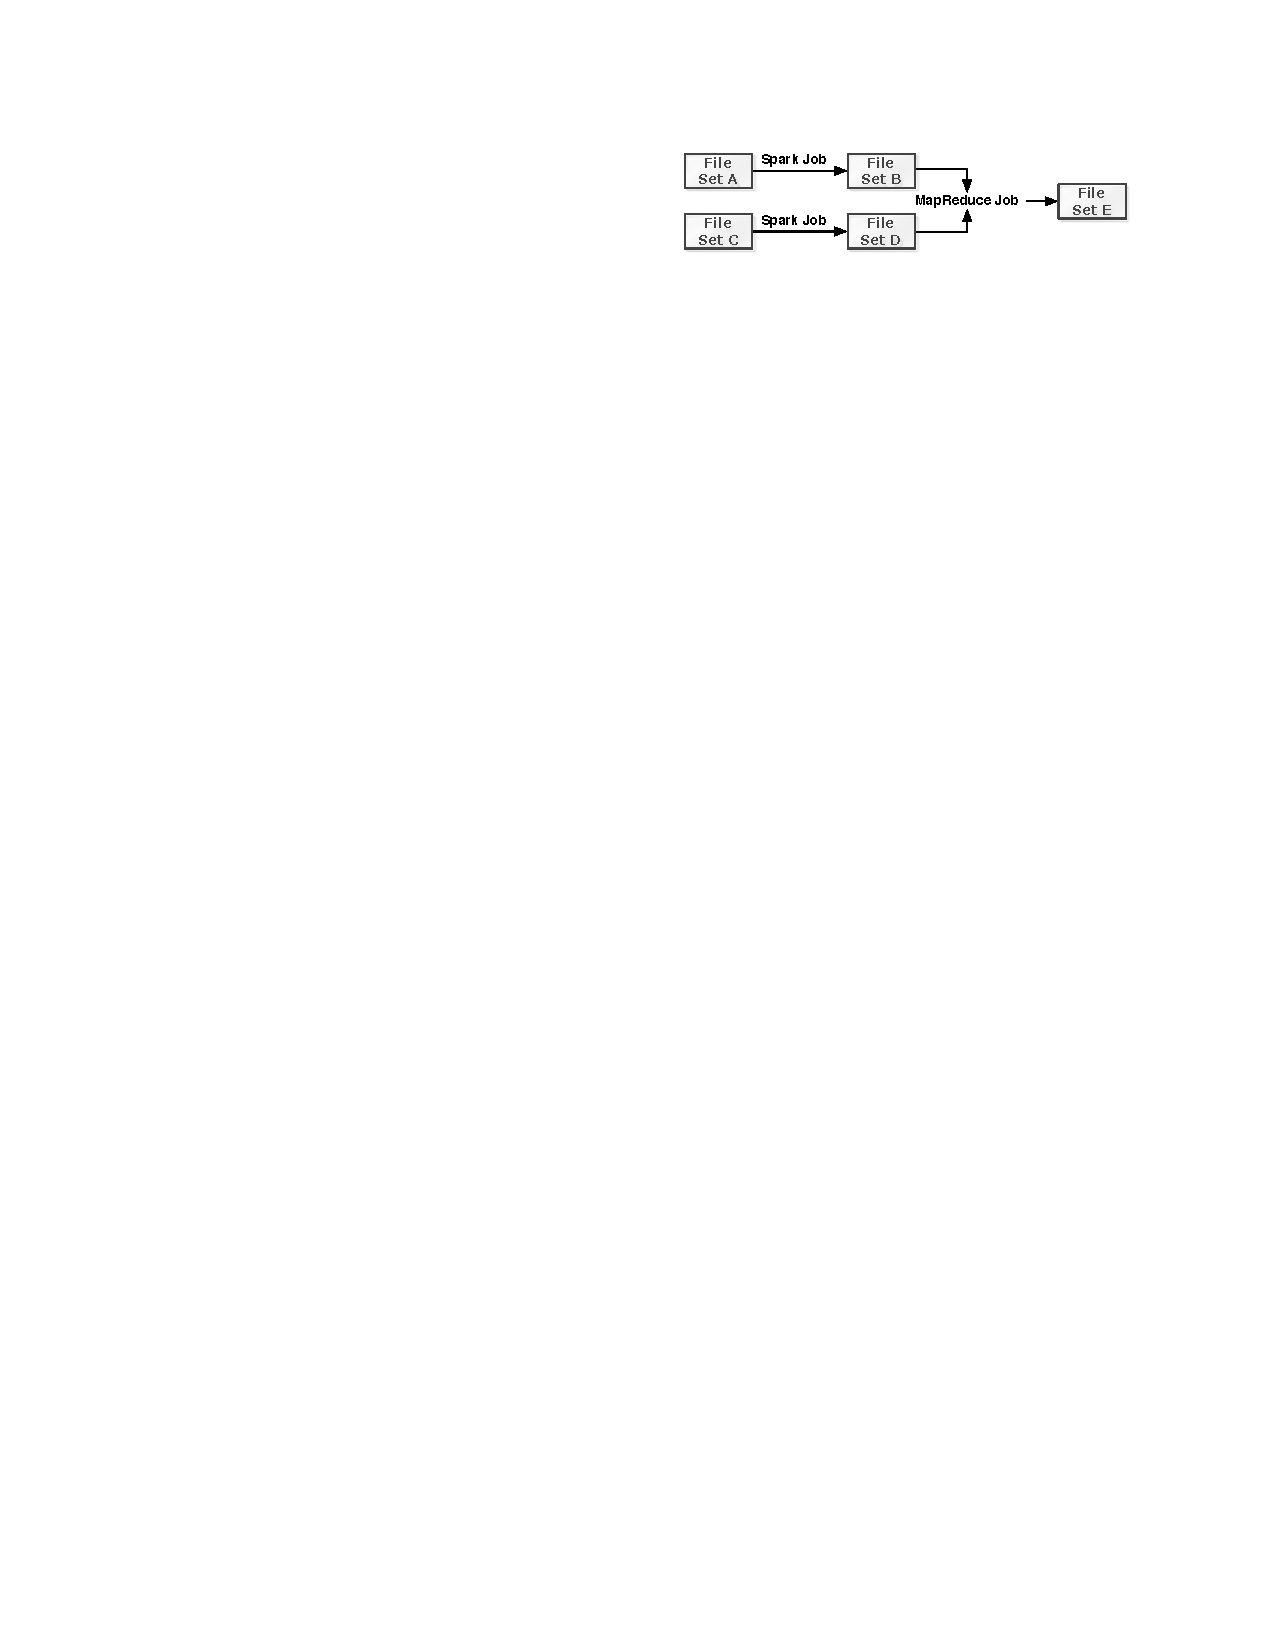
\includegraphics[width=0.48\textwidth]{lineage_graph.pdf}
        \caption{An Example of Lineage Graph.}
        \label{fig:lineage_graph}
\end{figure} 

BAD-FS separates out a scheduler from storage, which provides external control to the scheduler. 
Users submit jobs to the scheduler through a declarative workflow language, 
and thus the system knows the \textit{lineage} among jobs. 
However, to make this practical for parallel big data engines (e.g. Spark, MapReduce, Tez), two fundamental issues stood out: (1) ensuring that the interaction between the scheduler and the storage system is correct, e.g. avoiding deadlocks/priority inversion, (2) bounding recomputation time, which otherwise in a \textit{24/7 system} can grow unbounded. 
For the first problem, Tachyon provides mechanisms that avoid \textit{deadlocks/priority inversion}, while respecting the policy of schedulers. For the second problem, Tachyon provides an \textit{asynchronous checkpointing} algorithm that exploits the structure of the lineage graph as shown in Figure \ref{fig:lineage_graph} to continuously perform checkpointing in the background to guarantee bounded recovery time.

\noindent
\textbf{Cluster Computation Frameworks}
Spark system presents a data abstraction for big data analytics, called \textit{resilient distributed dataset} (RDD), 
which is a coarse-grained deterministic immutable data structure with lineage-based fault-tolerance \cite{RDD:2012}. 
On top of Spark, Spark SQL, Spark Streaming, MLlib and GraphX are built for SQL-based manipulation, stream processing, machine learning and graph processing, respectively. It has two main features:

\begin{itemize}
\item
  It uses an \textit{elastic persistence model} to provide the flexibility to
  persist the dataset in memory, on disks or both. By persisting the
  dataset in memory, it favors applications that need to read the
  dataset multiple times (e.g., iterative algorithms), and enables
  interactive queries.
\item
  It incorporates a \textit{light-weight fault-tolerance mechanism} (i.e., lineage), without the need for checkpointing. 
  The lineage of an RDD contains sufficient information such that it can be re-computed based on its lineage and dependent RDDs, which are the input data files in HDFS in the worst case. 
This  idea is also adopted by \emph{Tachyon}, which is a distributed file system enabling reliable file sharing via memory.
\end{itemize}
 
Spark uses \textit{lineage information} within a single job or shell, all running inside a single JVM. 
Different queries in Spark cannot share datasets (RDD) in a reliable and high-throughput fashion, 
because Spark is a computation engine, rather than a storage system. 
The integration of Tachyon with Spark substantially improves existing industry workflows of Spark jobs, 
as they can share datasets reliably through Tachyon. 
Moreover, Spark can benefit from the asynchronous checkpointing in Tachyon, which enables high-throughput write.
Other frameworks, such as MapReduce and Dryad, also trace task lineage within a job. 
However, as execution engines, they do not trace relations among files, 
and therefore can not provide high throughput data sharing among different jobs. 
Like Spark, they can also integrate with Tachyon to improve the efficiency of data sharing among different jobs or frameworks.

\noindent
\textbf{Caching Systems}
Cache plays an important role in enhancing system performance, especially in web applications. 
Facebook, Twitter, Wikipedia, LiveJournal, et al. are all taking advantage of cache extensively to provide good service. 
Cache can provide two optimizations for applications: optimization for \textit{disk I/O} by allowing to access data from
memory, and optimization for \textit{CPU workload} by keeping results without the need for re-computation. 
Many cache systems have been developed for various objectives.
Like Tachyon, Nectar also uses the concept of lineage, but it does so only for a specific programming framework (DryadLINQ), and in the context of a traditional, replicated file system. 
Nectar is a data reuse system for DryadLINQ queries whose goals are to save space and to avoid redundant computations. The former goal is achieved by deleting largely unused files and rerunning the jobs that created them when needed. However, no time bound is provided to retrieve deleted data. The latter goal is achieved by identifying pieces of code that are common in different programs and reusing previously computed files. Nectar achieves this by heavily resting on the SQL like DryadLINQ query semantics—in particular, it needs to analyze LINQ code to determine when results may be reused— and stores data in a replicated on-disk file system rather than attempting to speed up data access. In contrast, Tachyon’s goal is to provide data sharing across different frameworks with memory speed and bounded recovery time.

\begin{figure}[htb]
        \centering
        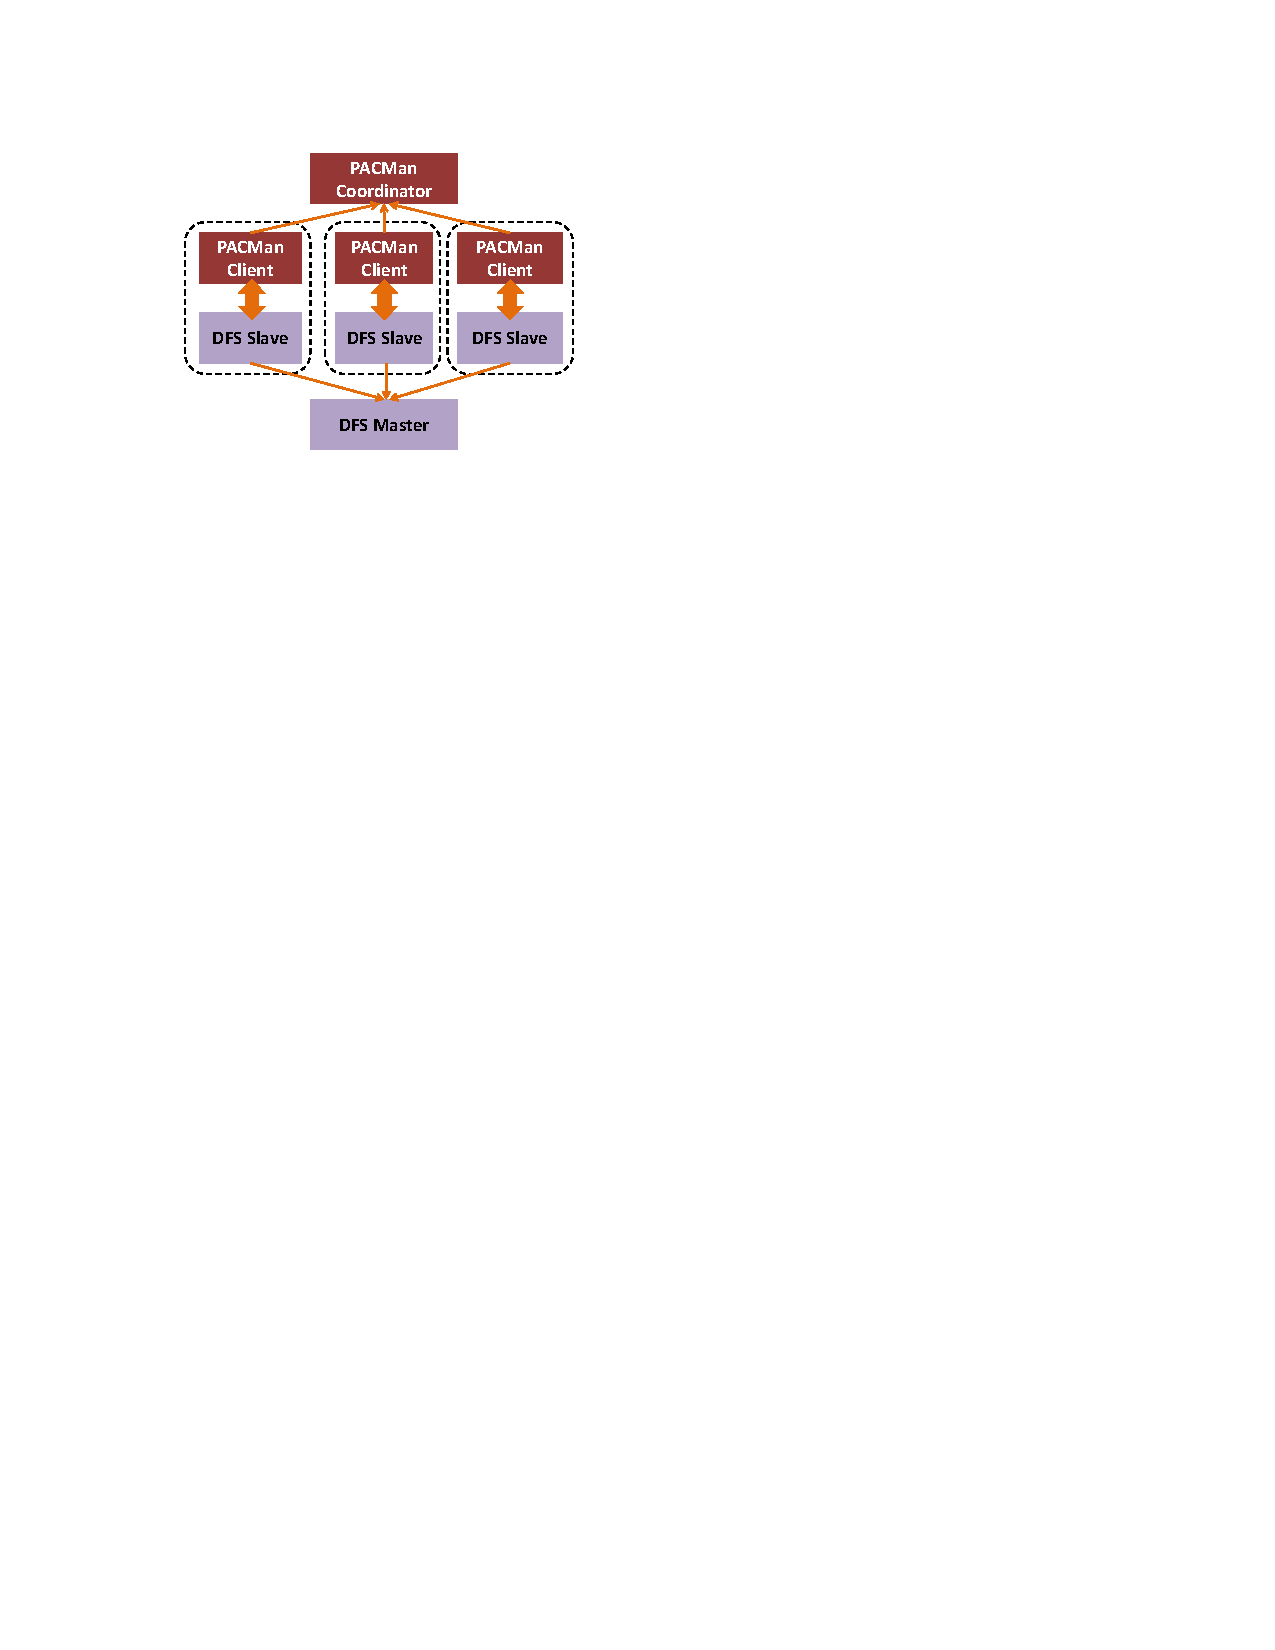
\includegraphics[width=0.48\textwidth]{pacman.pdf}
        \caption{PACMan Architecture. The central \textit{coordinator} manages the distributed clients. Thick arrows represent data flow while thin arrows denote meta-data flow.}
        \label{fig:pacman}
\end{figure} 

PACMan \cite{Anan:2012} is a \textit{memory caching system} for data-intensive parallel jobs (Figure \ref{fig:pacman}). It explores different policies to make data warehouse caching efficient. However, PACMan does not improve the performance of writes, nor the first read of any data item. Therefore, the throughput of many applications remains disk-limited—for example, a multi-job MapReduce workflow will still need to replicate data at disk speed between each step.
Lineage besides the applications in the above fields, lineage has been applied in other areas, such as scientific computing, databases, and distributed computing, for applications such as providing the history of data, which can be used for accountability, security, and data audit. Tachyon applies lineage in a different environment to achieve memory throughput read and write, which entails a different set of challenges.


\section{RAMCloud}
RAMCloud is a \textit{distributed in-memory key-value store}, featured for low latency, high availability and high memory utilization \cite{Ousterhout:2015}. In particular, it can achieve tens of microseconds latency
by taking advantage of low-latency networks (e.g., Infiniband and
Myrinet), and provide ``continuous availability'' by harnessing large
scale to recover in 1-2 seconds from system failure. In addition, it
adopts a log-structured data organization with a two-level cleaning
policy to structure the data both in memory and on disks. This results
in high memory utilization and a single unified data management
strategy. The architecture of RAMCloud consists of a coordinator who
maintains the metadata in the cluster such as cluster membership, data
distribution, and a number of storage servers, each of which contains
two components, a master module which manages the in-memory data and
handles read/write requests from clients, and a backup module which uses
local disks or flash memory to backup replicas of data owned by other
servers (Figure \ref{fig:ramcloud_architecture}).

\begin{figure}[htb]
        \centering
        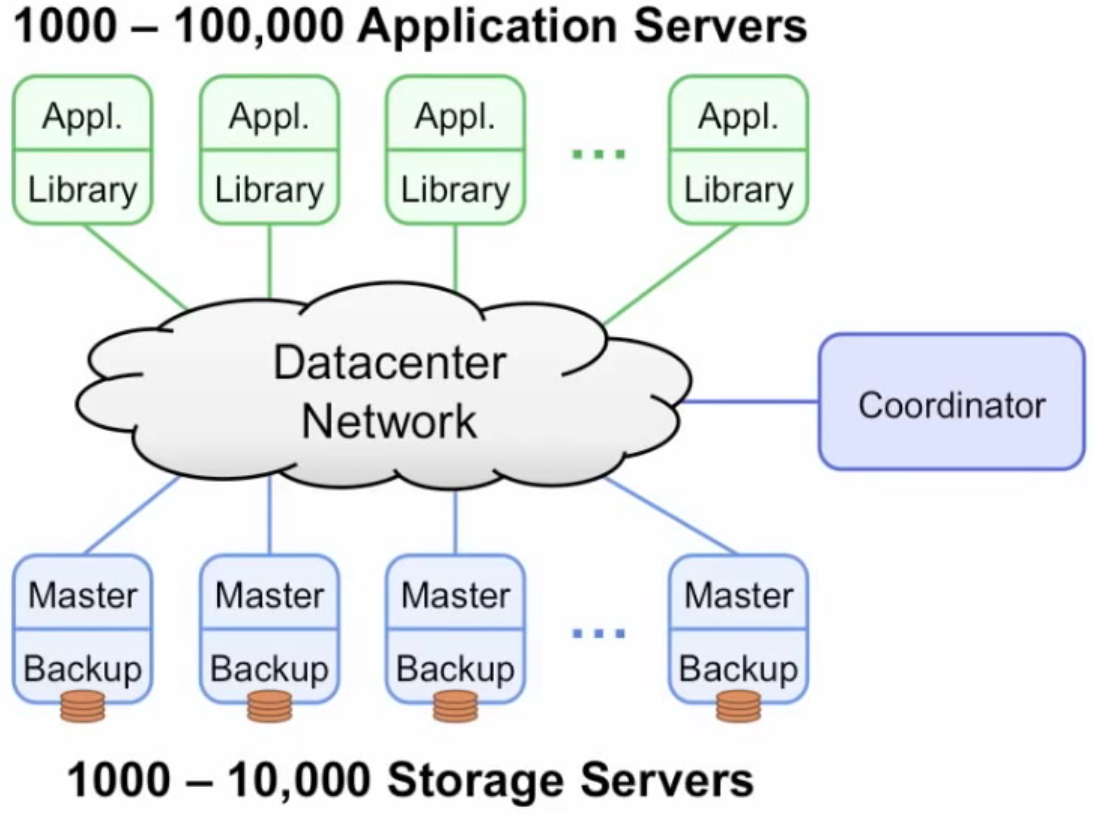
\includegraphics[width=0.48\textwidth]{architecture_ramcloud.png}
        \caption{RAMCloud Architecture}
        \label{fig:ramcloud_architecture}
\end{figure}

\noindent
\textbf{\emph{Data organization}}. Key-value objects in RAMCloud are grouped into
a set of tables, each of which is individually range-partitioned into a
number of tablets based on the hash-codes of keys. RAMCloud relies on
the uniformity of hash function to distribute objects in a table evenly
in proportion to the amount of hash space (i.e., the range) a storage
server covers. A storage server uses a single log to store the data, and
a hash table for indexing. Data is accessed via the hash table, which
directs the access to the current version of objects.

RAMCloud adopts a log-structured approach of memory management rather
than traditional memory allocation mechanisms (e.g., C library's
\emph{malloc}), allowing 80-90 percent memory utilization by eliminating
memory fragmentation. In particular, a log is divided into a set of
\emph{segments}. As the log structure is append-only, objects are not
allowed to be deleted or updated in place. Thus a periodic clean job
should be scheduled to clean up the deleted/stale objects to reclaim
free space. RAMCloud designs an efficient two-level cleaning policy.

\begin{itemize}
\item
  It schedules a \emph{segment compaction} job to clean the log segment
  in memory first whenever the free memory is less than 10 percent, by
  copying its live data into a smaller \emph{segment} and freeing the
  original \emph{segment}.
\item
  When the data on disk is larger than that in memory by a threshold, a
  \emph{combined cleaning} job starts, cleaning both the log in memory
  and on disk together.
\end{itemize}

A two-level cleaning policy can achieve a high memory utilization by
cleaning the in-memory log more frequently, and meanwhile reduce disk
bandwidth requirement by trying to lower the disk utilization (i.e.,
increase the percentage of deleted/stale data) since this can avoid
copying a large percentage of live data on disk during cleaning (Figure \ref{fig:buffered_logging}).

\noindent
\textbf{\emph{Fast crash recovery}}. One big challenge for in-memory storage is
fault-tolerance, as the data is resident in the volatile
DRAM. 
RAMCloud uses replication to guarantee durability by replicating data in remote disks,
and harnesses the large scale of resources (e.g., CPU, disk bandwidth)
to speed up recovery process. Specifically, when receiving an update
request from a client, the master server appends the new object to the
in-memory log, and then forwards the object to \emph{R} (usually
\emph{R} = 3) remote backup servers, which buffer the object in memory
first and flush the buffer onto disk in a batch (i.e., in unit of
\emph{segment}). The backup servers respond as soon as the object has
been copied into the buffer, thus the response time is dominated by the
network latency rather than the disk I/O.

To make recovery faster, replicas of the data are scattered across all
the backup servers in the cluster in unit of \emph{segment}, thus making
more backup servers collaborate for the recovery process. Each master
server decides independently where to place a segment replica using a
combination of randomization and refinement, which not only eliminates
pathological behaviors but also achieves a nearly optimal solution.
Furthermore, after a server fails, in addition to all the related backup
servers, multiple master servers are involved to share the recovery job
(i.e., re-constructing the in-memory log and hash table), and take
responsibility for ensuring an even partitioning of the recovered data.
The assignment of recovery job is determined by a \emph{will} made by
the master before it crashes. The \emph{will} is computed based on
\emph{tablet profiles}, each of which maintains a histogram to track the
distribution of resource usage (e.g., the number of records and space
consumption) within a single table/tablet. The \emph{will} aims to
balance the partitions of a recovery job such that they require roughly
equal time to recover.

\begin{figure}[htb]
        \centering
        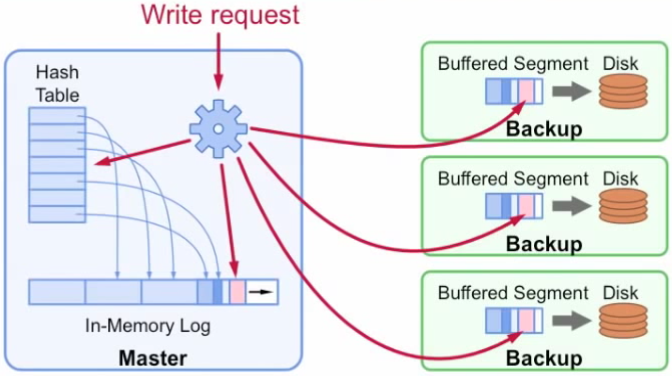
\includegraphics[width=0.48\textwidth]{buffered_logging.png}
        \caption{Buffered Logging Approach}
        \label{fig:buffered_logging}
\end{figure}

The random replication strategy produces almost uniform allocation of
replicas and takes advantage of the large scale, thus preventing data
loss and minimizing recovery
time. However,
this strategy may result in data loss under simultaneous node failures. 
Although the amount of lost data may
be small due to the high dispersability of segment replicas, it is
possible that all replicas of certain part of the data may become
unavailable. 
Hence RAMCloud
also supports another replication mode based on \emph{Copyset}, to reduce the probability of data loss
after large, coordinated failures such as power loss. Copyset trades off
the amount of lost data for the reduction in the frequency of data loss,
by constraining the set of backup servers where all the segments in a
master server can be replicated to. However, this can lead to longer
recovery time as there are fewer backup servers for reading the replicas
from disks. The trade-off can be controlled by the scatter width, which
is the number of backup servers that each server's data are allowed to
be replicated to. For example, if the scatter width equals the number of
all the other servers (except the server that wants to replicate) in the
cluster, Copyset then turns to random replication.

\section{Tachyon}
Tachyon is a \textit{memory-centric fault-tolerant distributed storage system}, which enables reliable file sharing at memory-speed across cluster frameworks such as Spark and MapReduce. 
Tachyon is Hadoop compatible. Existing Spark and MapReduce programs can run on top of it without any code changes. Tachyon is the default off-heap option in Spark, which means that RDDs can automatically be stored inside Tachyon to make Spark more resilient and avoid GC overheads. 

\begin{figure}[htb]
        \centering
        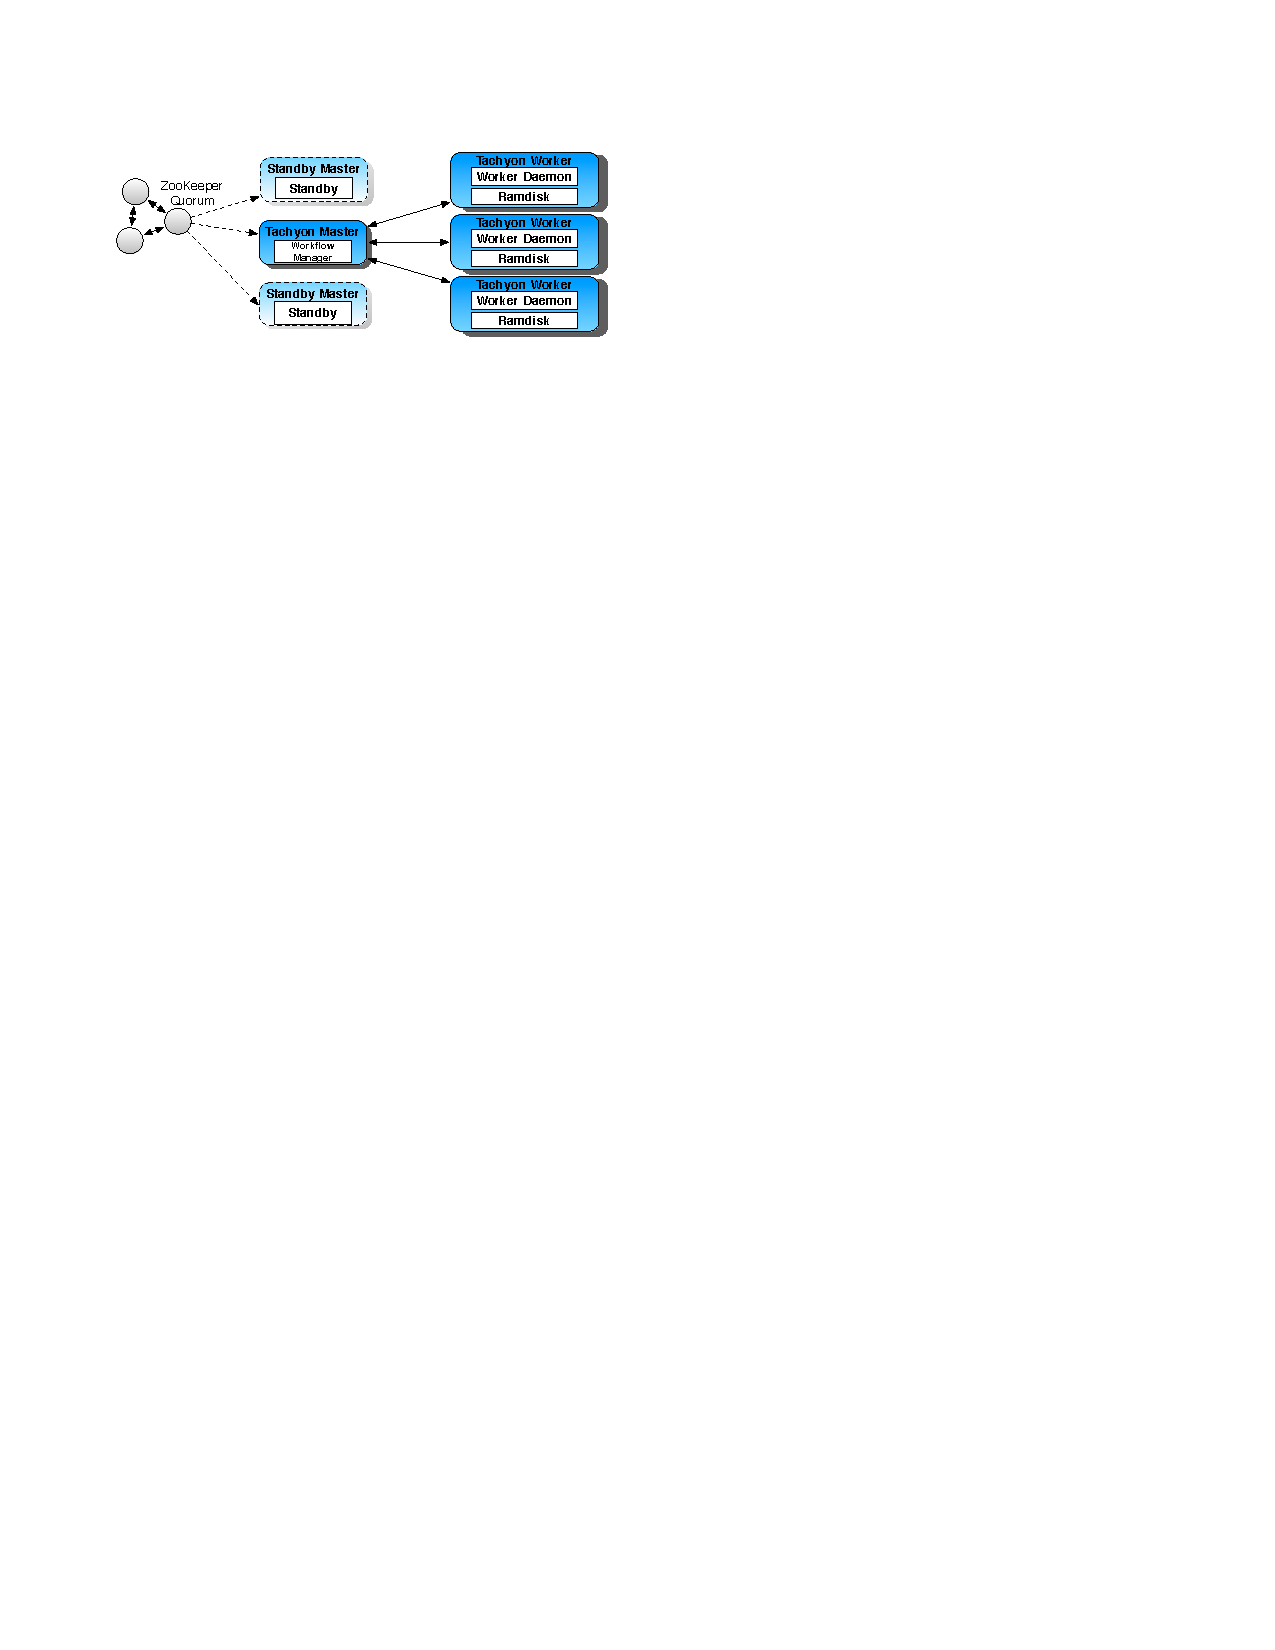
\includegraphics[width=0.48\textwidth]{tachyon_architecture.pdf}
        \caption{Tachyon Architecture}
        \label{fig:tachyon_architecture}
\end{figure}

Tachyon consists of two layers: \textit{lineage} and \textit{persistence}. The lineage layer provides high throughput I/O and tracks the sequence of jobs that have created a particular data output. The persistence layer persists data onto storage without the lineage concept. This is mainly used to do asynchronous checkpoints. The persistence layer can be any existing replication based storage systems, such as HDFS, S3, Glusterfs.

Tachyon employs a standard master-slave architecture similar to HDFS and GFS as shown in Figure \ref{fig:tachyon_architecture}.
In addition to managing metadata, the master also contains a \textit{workflow manager}. 
The role of this manager is to track lineage information, compute \textit{checkpoint order}, and interact with a cluster resource manager to allocate resources for \textit{recomputation}.
Each worker runs a daemon that manages local resources, and periodically reports the status to the master. 
In addition, each worker uses a RAMdisk for storing \textit{memory-mapped files}. A user application can bypass the daemon and interact directly with RAMdisk. This way, an application with \textit{data locality} can interact with data at memory speeds, while avoiding any extra data copying.

\begin{figure}[htb]
        \centering
        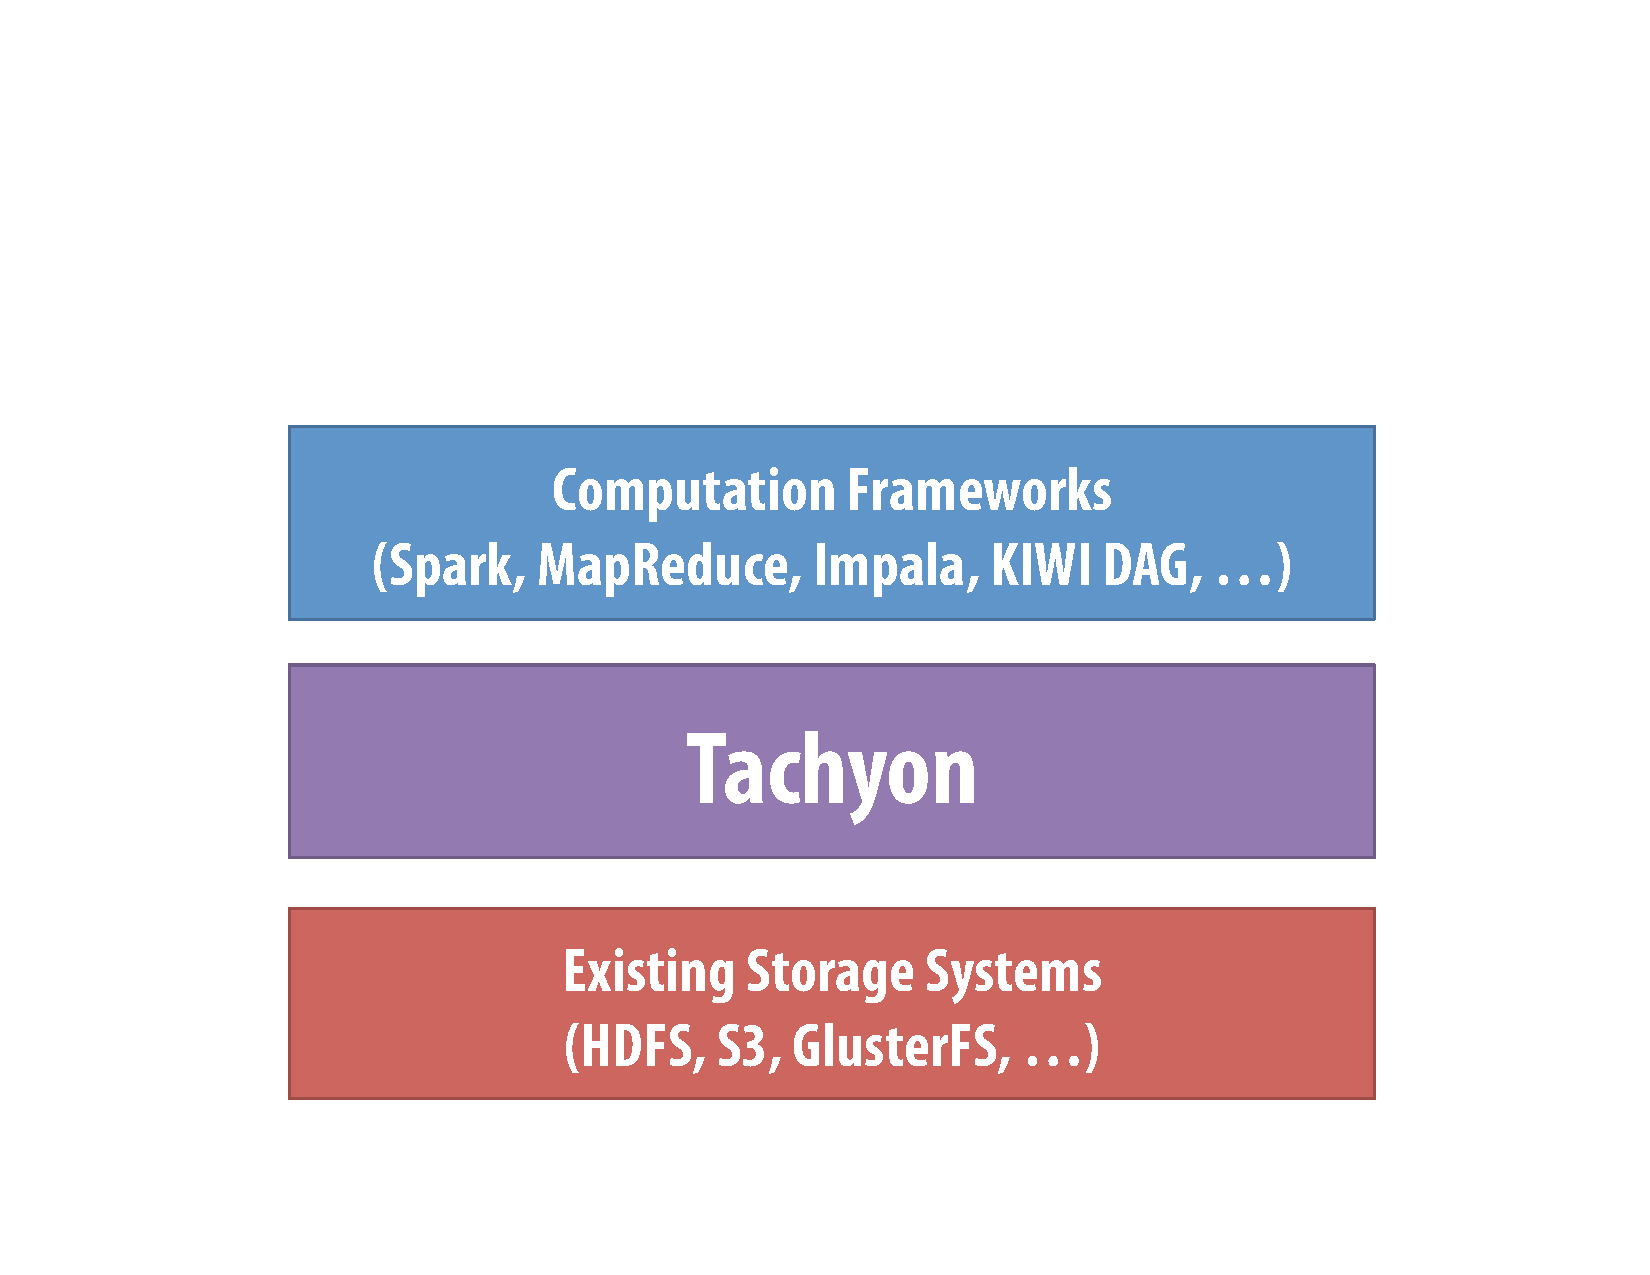
\includegraphics[width=0.48\textwidth]{stack.pdf}
        \caption{Tachyon Integration Stack}
        \label{fig:tachyon_stack}
\end{figure}

Tachyon implements the Hadoop FileSystem interface. Therefore, Hadoop MapReduce and Spark can run with Tachyon without modification. However, close integration is required to fully take advantage of Tachyon, and we are working towards that. End-to-end latency speedup depends on the workload and the framework, since various frameworks have different execution overhead.

Tachyon’s native API is similar to that of the \texttt{java.io.File} class, providing InputStream and OutputStream interfaces and efficient support for memory-mapped I/O. We recommend using this API to get the best performance from Tachyon.
To provide fault-tolerance, Tachyon checkpoints in-memory data to the underlayer file system. It has a generic interface to make plugging different underlayer file systems easy. We currently support HDFS, S3, GlusterFS, and single-node local file systems (Figure \ref{fig:tachyon_stack}).

Table data with over hundreds of columns is common in data warehouses. Tachyon provides native support for multi-columned data, with the option to put only hot columns in memory to save space.
Users can browse the file system easily through the web UI. Under debug mode, administrators can view detailed information of each file, including locations, checkpoint path, etc.
Users can use \texttt{./bin/tachyon tfs} to interact with Tachyon, e.g. copy data in and out of the file system.

\section{Conclusion}
As memory becomes the new disk, in-memory data management and processing becomes increasingly interesting for both academia and industry.
Shifting the data storage layer from disks to main memory can lead to more than 100$\times$ theoretical improvement in terms of response time and throughput. 
As ever more datacenter workloads start to be in memory, write throughput becomes a major bottleneck for applications. Therefore, we believe that lineage-based recovery might be the only way to speed up cluster storage systems to achieve memory throughput.

Tachyon is an open source project started in the UC Berkeley AMP Lab. 
Tachyon is high-throughput, fault-tolerant memory centric storage, with lineage as a first class citizen. 
We consider to use Tachyon as a staging storage at intermediate task execution step for efficient KIWI DAG execution.

\bibliographystyle{abbrv}
\bibliography{sqlonhadoop-2015-10}

\end{document}
